\appendix
\label{an_Datenblaetter}
\chapter{Datenblätter der untersuchten Energiespeicher}
\begin{figure}[h!]\centering
	%TODO: Kriege ich das Datenblatt
	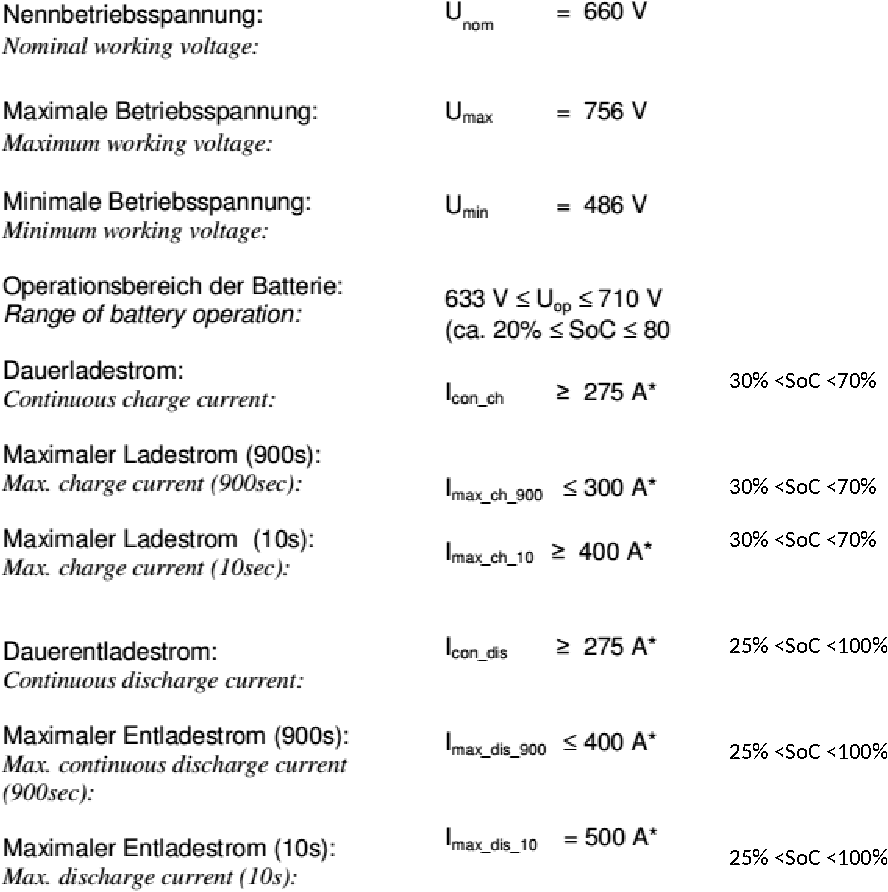
\includegraphics[height=15cm]{Datenblatt_LTO}
	\caption[Daten zum Primove-Akku]{Daten zum Primove-Akku. Quelle: MPM TU Berlin}
\end{figure}

\begin{figure}\centering
	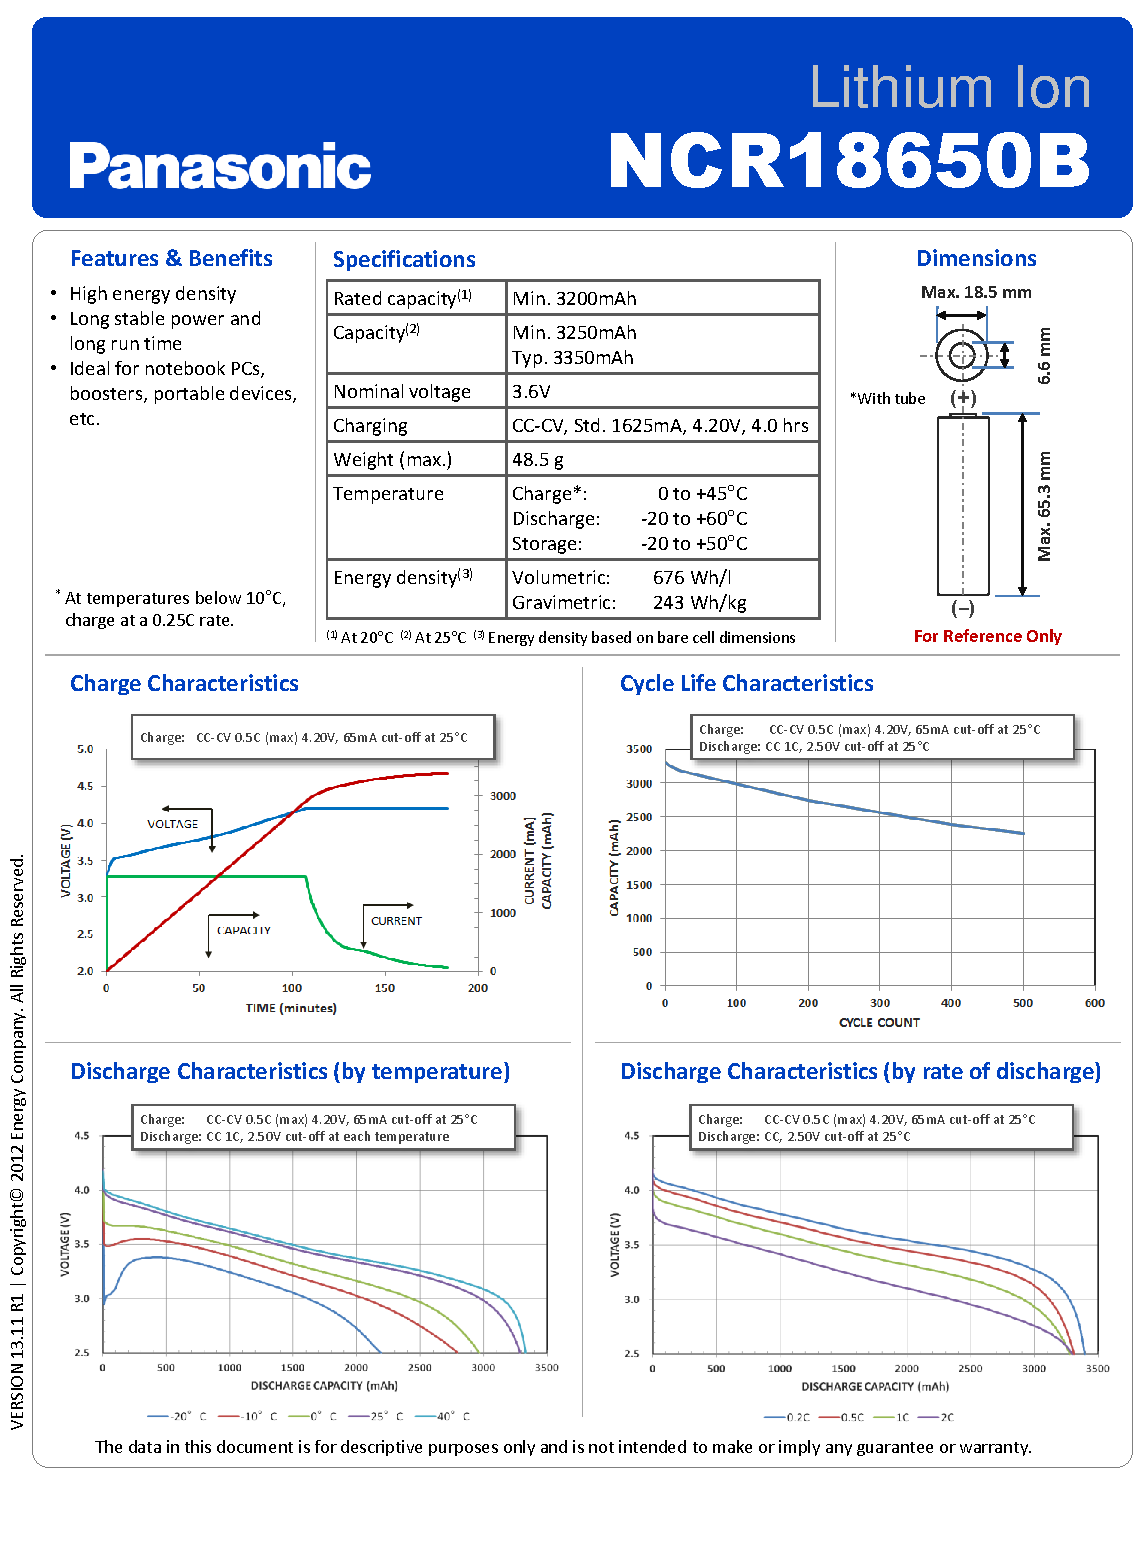
\includegraphics[height=20cm]{Datenblatt_18650}
	\caption[Datenblatt Panasonic NCR18650B]{Datenblatt Panasonic NCR18650B. Quelle: Panasonic Industrial North America}
\end{figure}

\begin{figure}\centering
	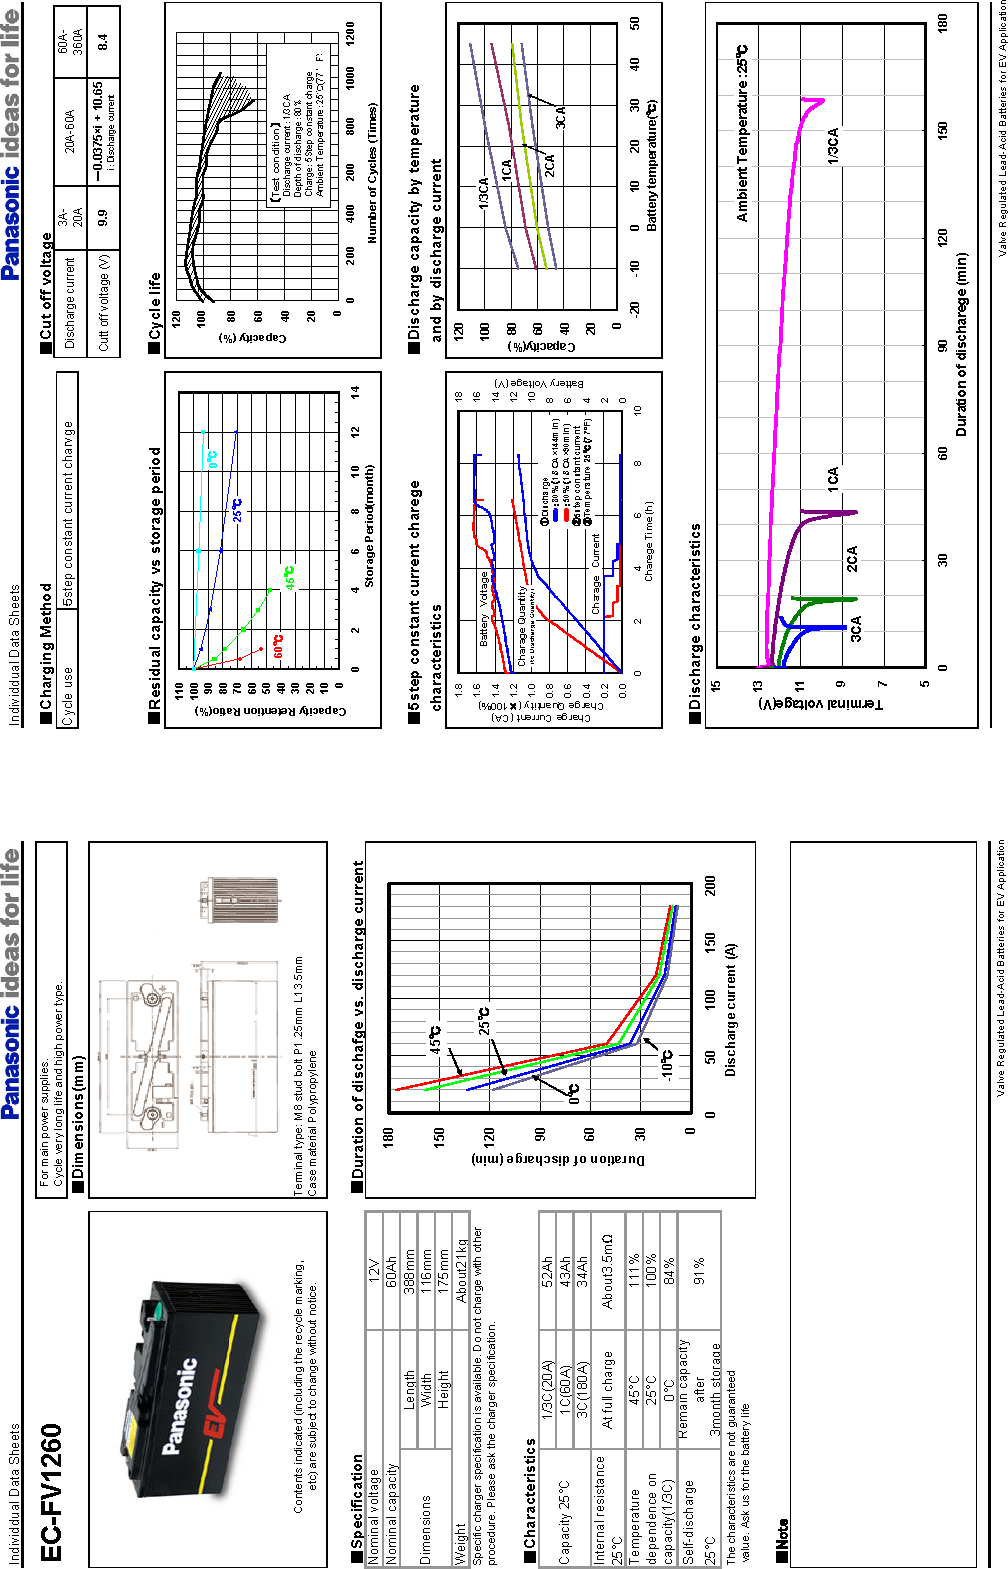
\includegraphics[height=20cm]{Datenblatt_VRLA}
	\caption[Datenblatt Panasonic EC-FV1260]{Datenblatt Panasonic EC-FV1260. Quelle: Panasonic Industrial North America}
\end{figure}

\begin{figure}\centering
	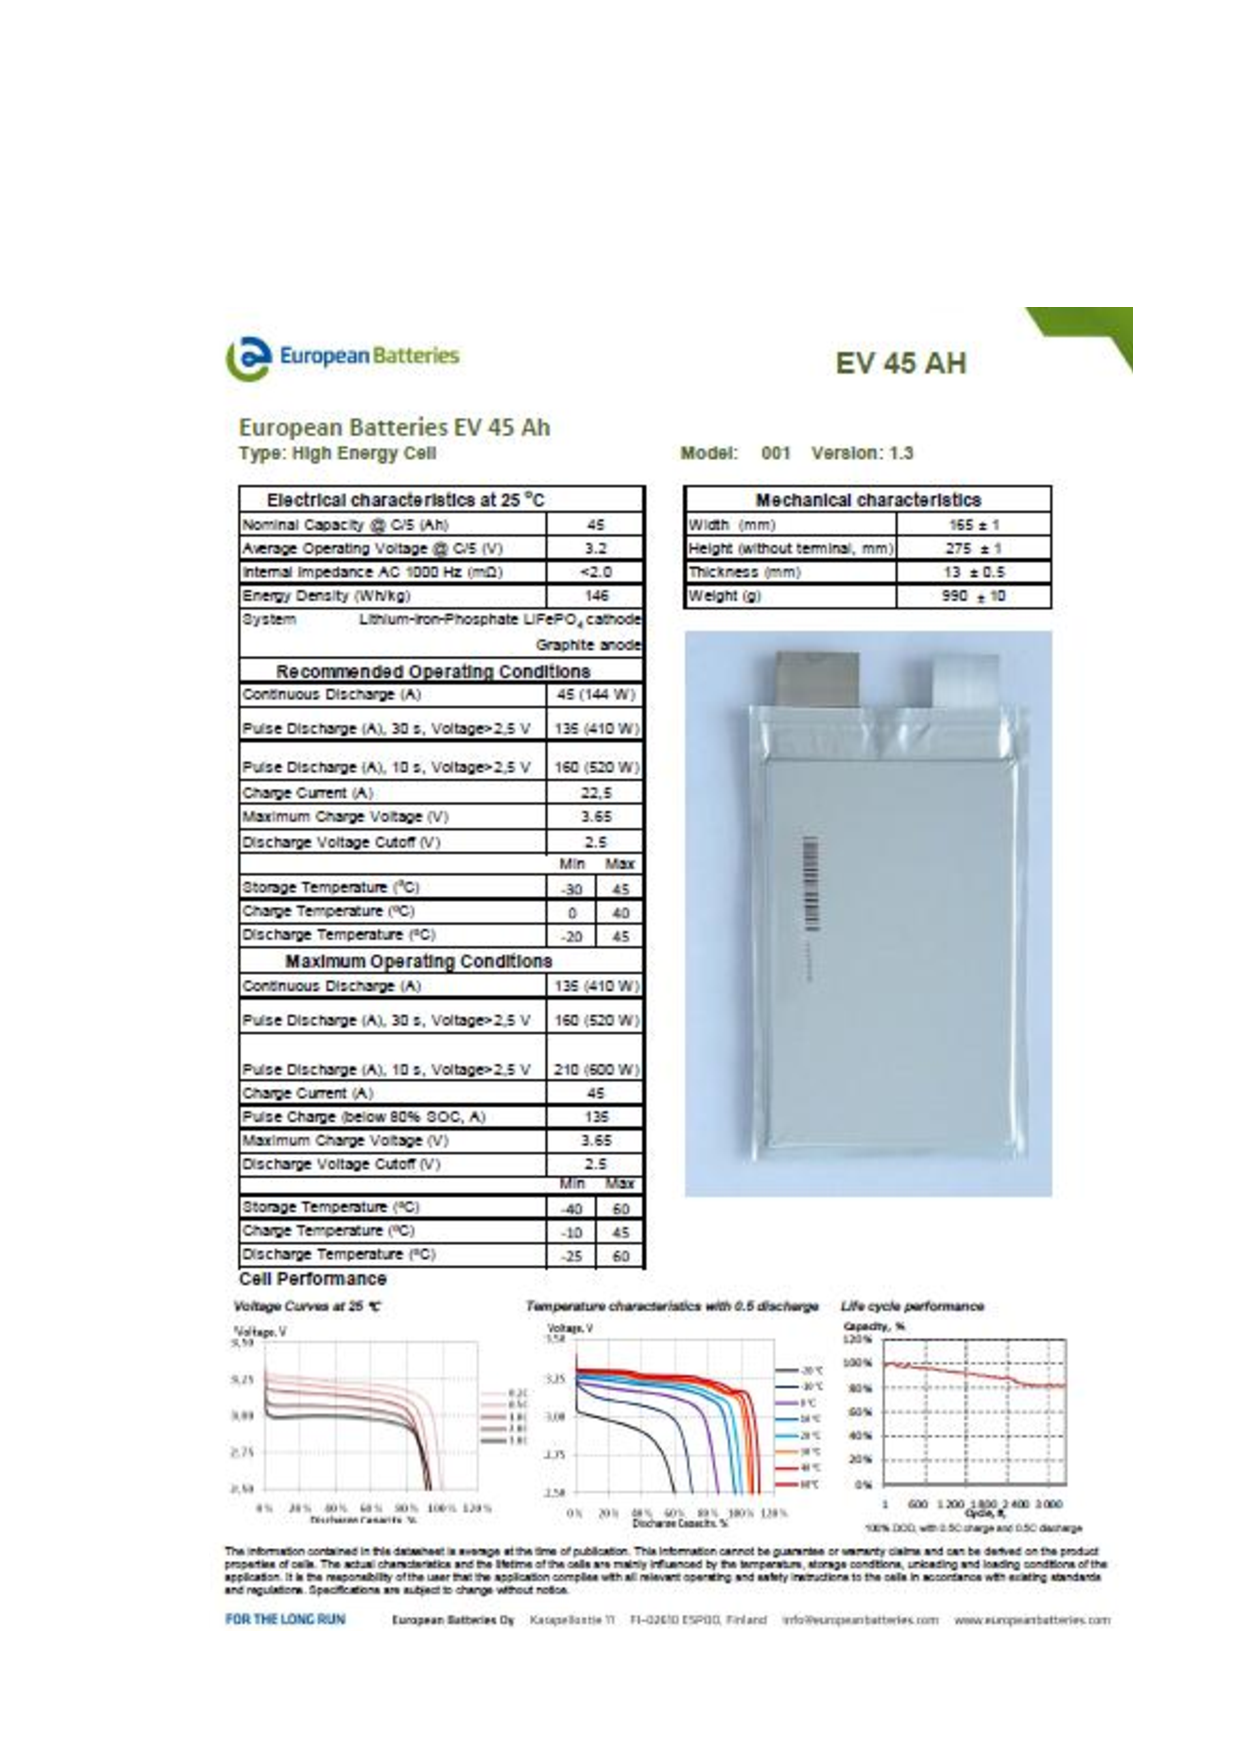
\includegraphics[height=20cm]{Datenblatt_LFP}
	\caption[Datenblatt European Batteries LiFePO EV 45 Ah]{Datenblatt European Batteries LiFePO EV 45 AH. Quelle: SuperLIB Deliverable 4.1 – Cell Specification with Cell Data}
\end{figure}

\begin{figure}\centering
	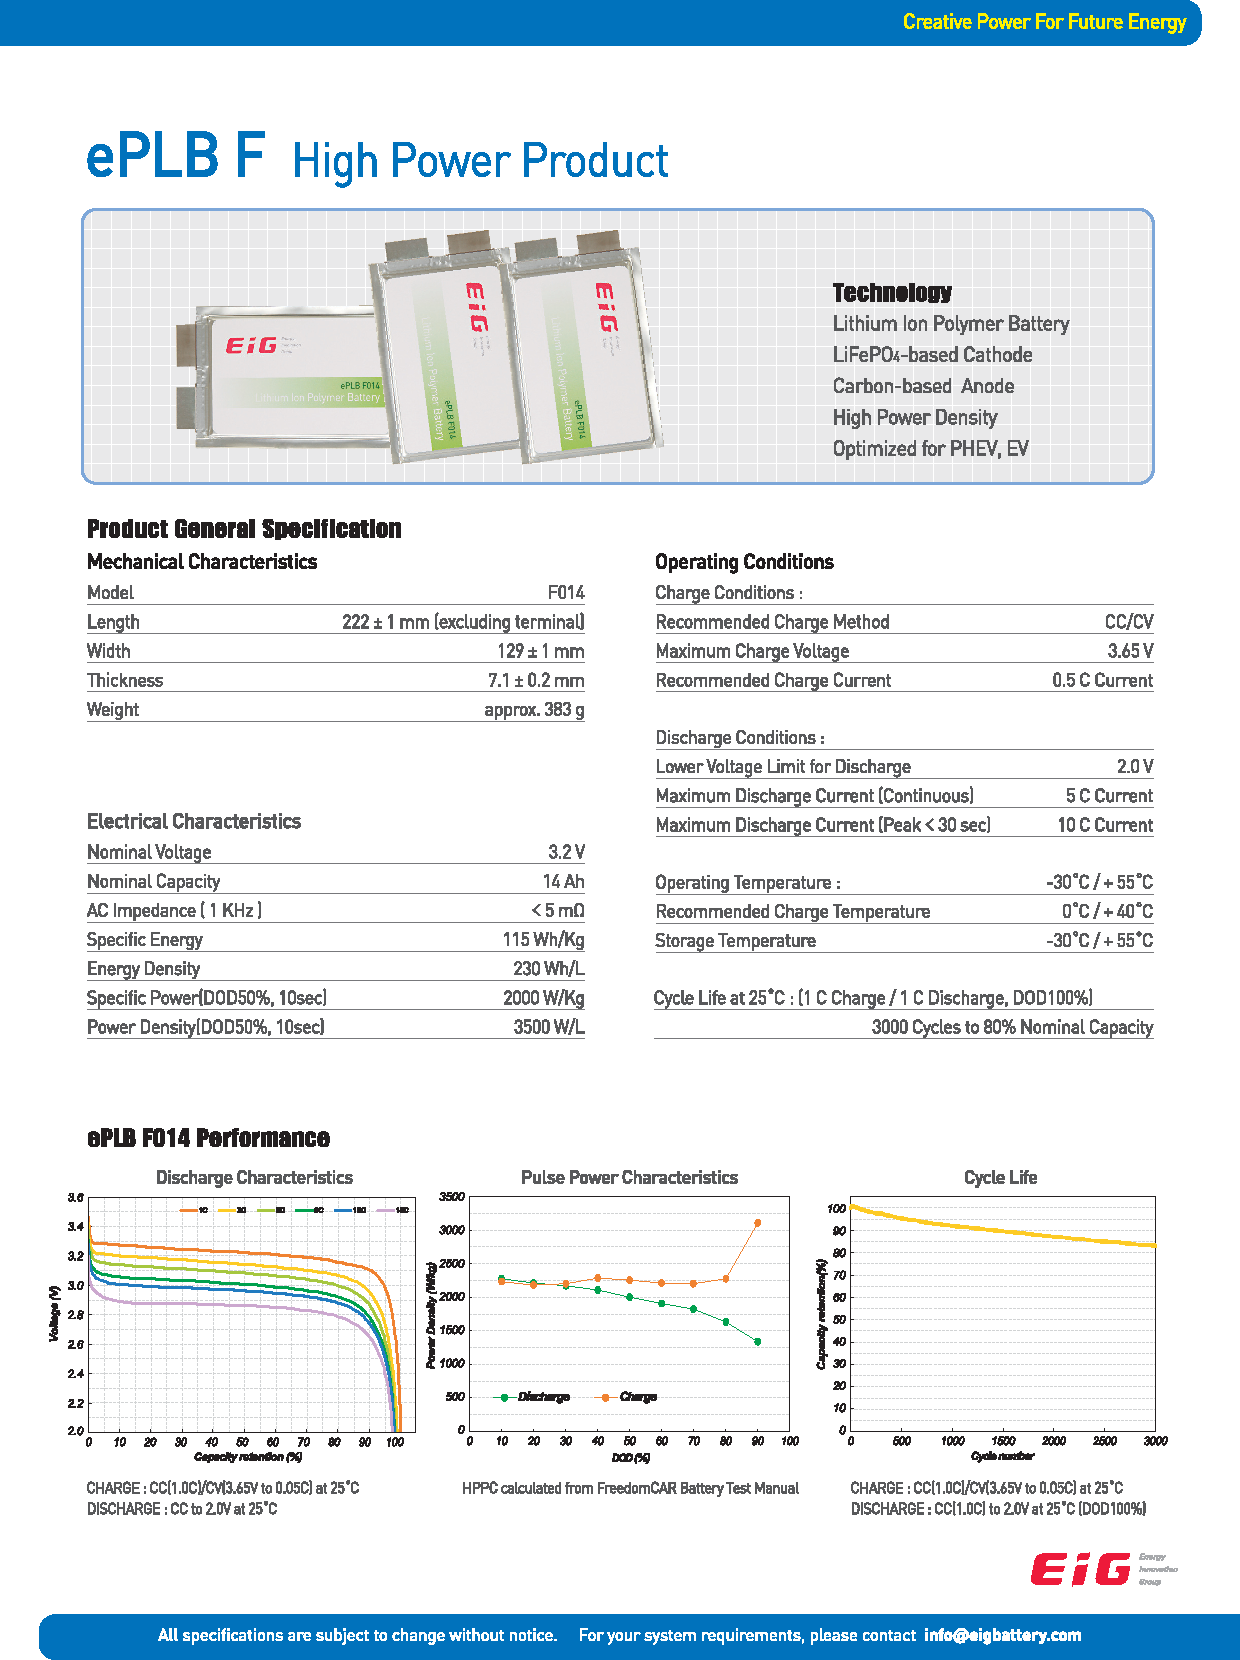
\includegraphics[height=20cm]{Datenblatt_LFP_HP}
	\caption[Datenblatt EIG ePLB F 14 Ah]{Datenblatt EIG ePLB F 14Ah. Quelle: SuperLIB Deliverable 4.1 – Cell Specification with Cell Data}
\end{figure}